%%%%%%%%%%%%%%%%%%%%%%%%%%%%%%%%%%%%%%
%%%%%%%%%%%%%%%%%%%%%%%%%%%%%%%%%%%%%%
% Do not edit the TeX file your work
% will be overwritten.  Edit the RnW
% file instead.
%%%%%%%%%%%%%%%%%%%%%%%%%%%%%%%%%%%%%%
%%%%%%%%%%%%%%%%%%%%%%%%%%%%%%%%%%%%%%





\newcommand{\DefineMacros}{
\newcommand{\AlexNSur}{4,364}
\newcommand{\AlexNTar}{4,085,282}
\newcommand{\AlexSurmean}{0.462}
\newcommand{\AlexMrp}{0.288}
\newcommand{\AlexMrpSD}{0.0169}
\newcommand{\AlexRaking}{0.263}

}

%%%%%%%%%%%%%%%%%%%%%%
% Tables

\newcommand{\AlexanderBandFig}{

\begin{knitrout}
\definecolor{shadecolor}{rgb}{0.969, 0.969, 0.969}\color{fgcolor}\begin{figure}[!h]

{\centering 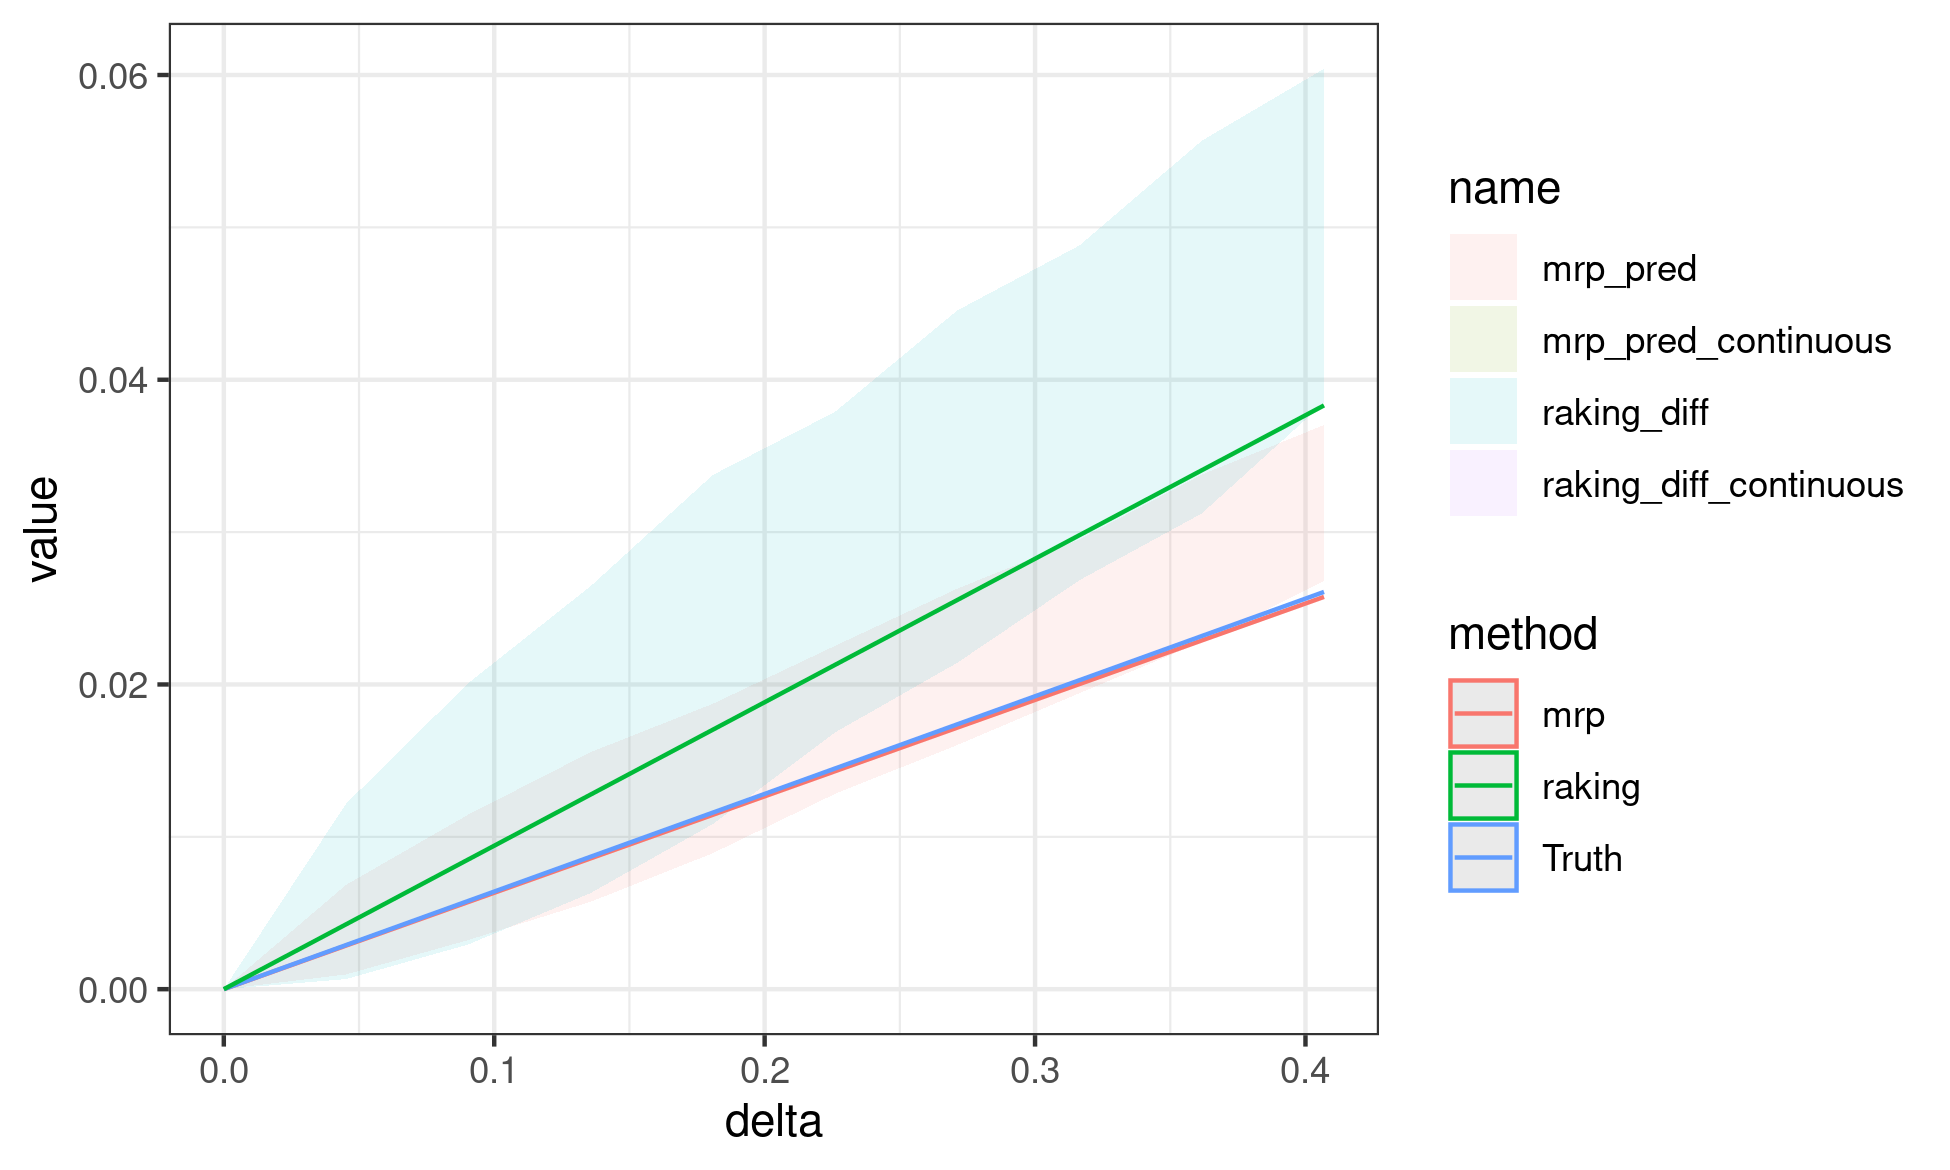
\includegraphics[width=0.98\linewidth,height=0.588\linewidth]{figure/alexanderbalance-1} 

}

\caption[Balance checks for Alexander]{Balance checks for Alexander}\label{fig:alexanderbalance}
\end{figure}

\end{knitrout}
}



\newcommand{\AlexanderImbalancePrimary}{

\begin{knitrout}
\definecolor{shadecolor}{rgb}{0.969, 0.969, 0.969}\color{fgcolor}\begin{figure}[!h]

{\centering 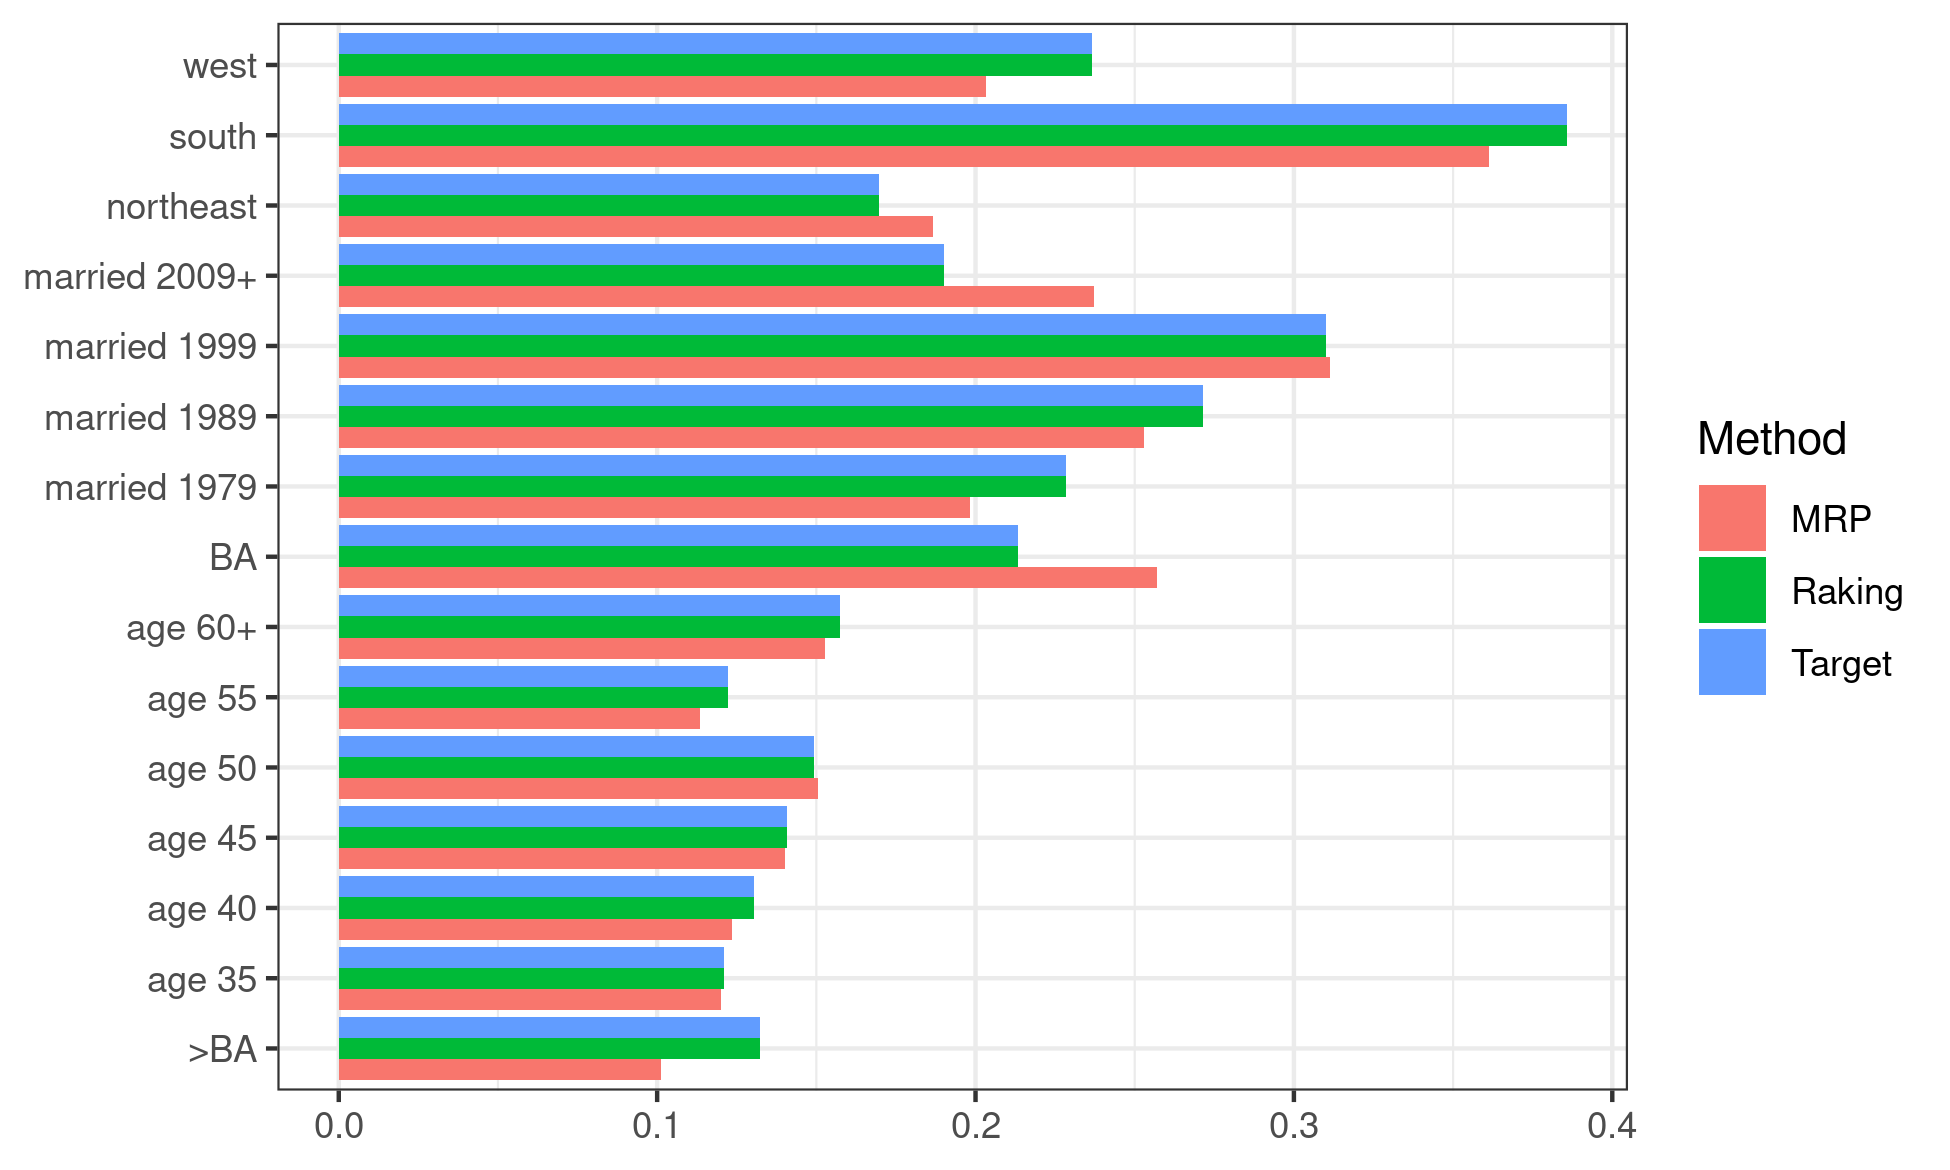
\includegraphics[width=0.98\linewidth,height=0.588\linewidth]{figure/alexanderprimary-1} 

}

\caption[Imbalance plot for primary effects]{Imbalance plot for primary effects}\label{fig:alexanderprimary}
\end{figure}

\end{knitrout}
}


\newcommand{\AlexanderImbalanceInteraction}{

\begin{knitrout}
\definecolor{shadecolor}{rgb}{0.969, 0.969, 0.969}\color{fgcolor}\begin{figure}[!h]

{\centering 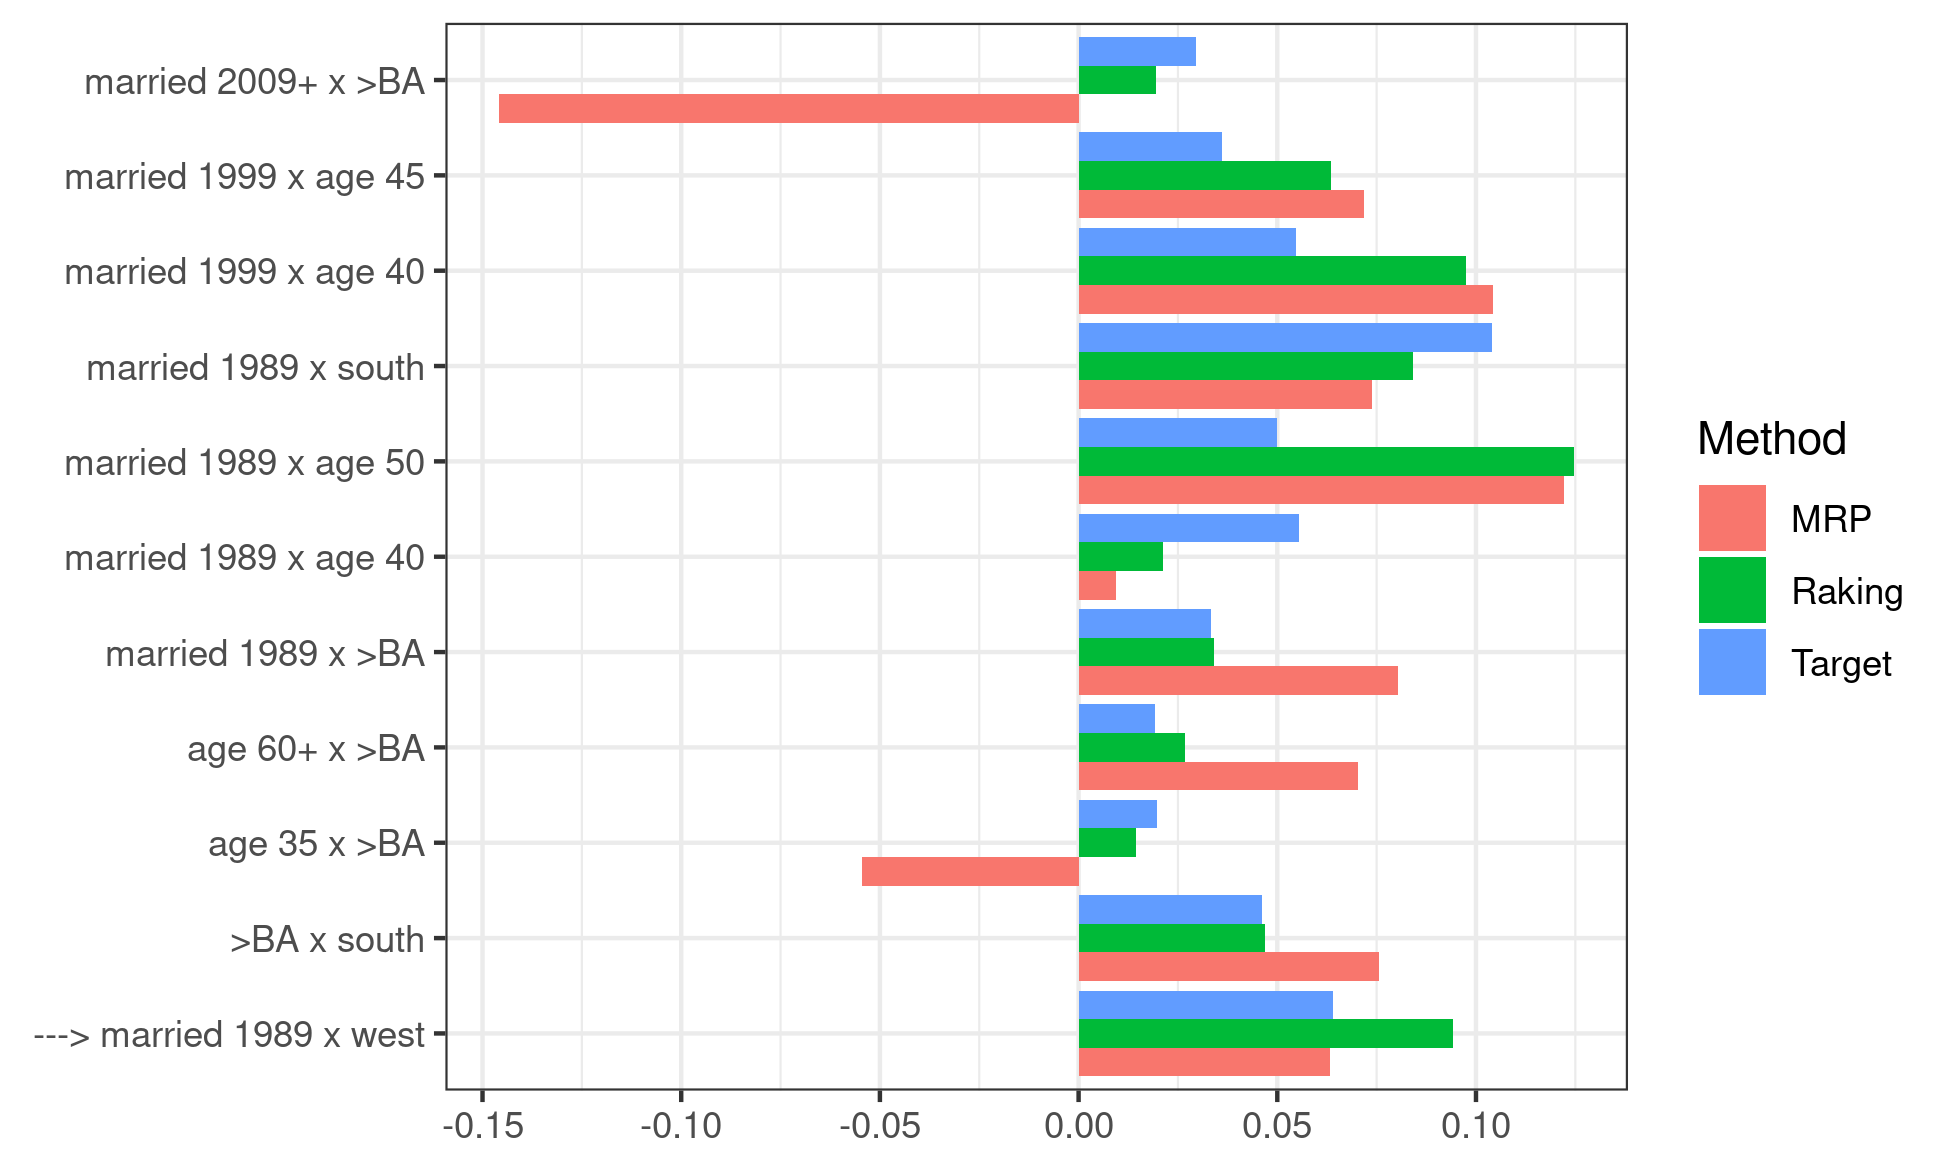
\includegraphics[width=0.98\linewidth,height=0.588\linewidth]{figure/alexanderinteraction-1} 

}

\caption[Imbalance plot for interaction effects]{Imbalance plot for interaction effects}\label{fig:alexanderinteraction}
\end{figure}

\end{knitrout}
}
